\documentclass[a4paper,10pt]{article}
\usepackage{fontspec}
\usepackage{setspace}
\usepackage{booktabs}
\usepackage{amsmath}
\usepackage{cancel}
\usepackage{graphicx}
\usepackage{biblatex}
\usepackage{float}
\usepackage{tabularx}
\usepackage{booktabs}

\setmainfont{arial}
\setstretch{1.15}
\addbibresource{refs.bib}

\title{GAN for Wild Fire Prediction}
\author{Arif Suganda, Riski Anggita \\
        Tadulako University
}

\begin{document}
\maketitle
\section{Problem Statement}
Climate change has increased the frequencies of wildfire and has been a quite challenging problem due to the risk and cost to monitor the spread of the wildfire. 
Advances in remote sensing and artificial intelligence provide new opportunities to improve detection capabilities. 
This experiment aims to offer a solution for this problem using a Generative Adversarial Network (GAN) integrated into an interface to identify an image as a wildfire or not. 
The solution aims to support researchers and disaster-management agencies with accessible, automated image analysis. 
\section{Dataset}
The dataset used in this research is Wildfire Prediction Dataset [1], a dataset of satellite images labeled by whether or not a wildfire event occurred. 
There are about 42,850 RGB images, with the size of 350 pixels times 350 pixels, labelled with 2 classes which represent areas that have experienced wildfires and those that have not.

The images were collected using the geographic coordinates of wildfire in Canada. 
Consisting of 22710 images of wildfire class and 20140 RGB images of no wildfire class. 
Dataset divided into train, test and validation with percentage of 70\% training data, 15\% testing data and 15\% validation data [24].

This setup helps build strong models and ensures fair evaluation. It is the main resource for training deep learning models in this study. 
Because it has a balanced mix of wildfire and non-wildfire images, the dataset helps the generator learn important visual features and allows the discriminator to tell the difference between real and generated images.

\section{Experiment}
This experiment is using generative adversarial network (GAN) to assist the prediction of wildfire class.
GAN model will create synthetic data to assist the CNN classifier model training using 20\% synthectic data as training dataset.
The purpose of synthetic data is to enrich the training dataset to improve the robustness and generalization of the classifier model.
The architecture of the GAN model can be seen in figure~\ref*{fig:gan}

\begin{figure}[H]
    \centering
    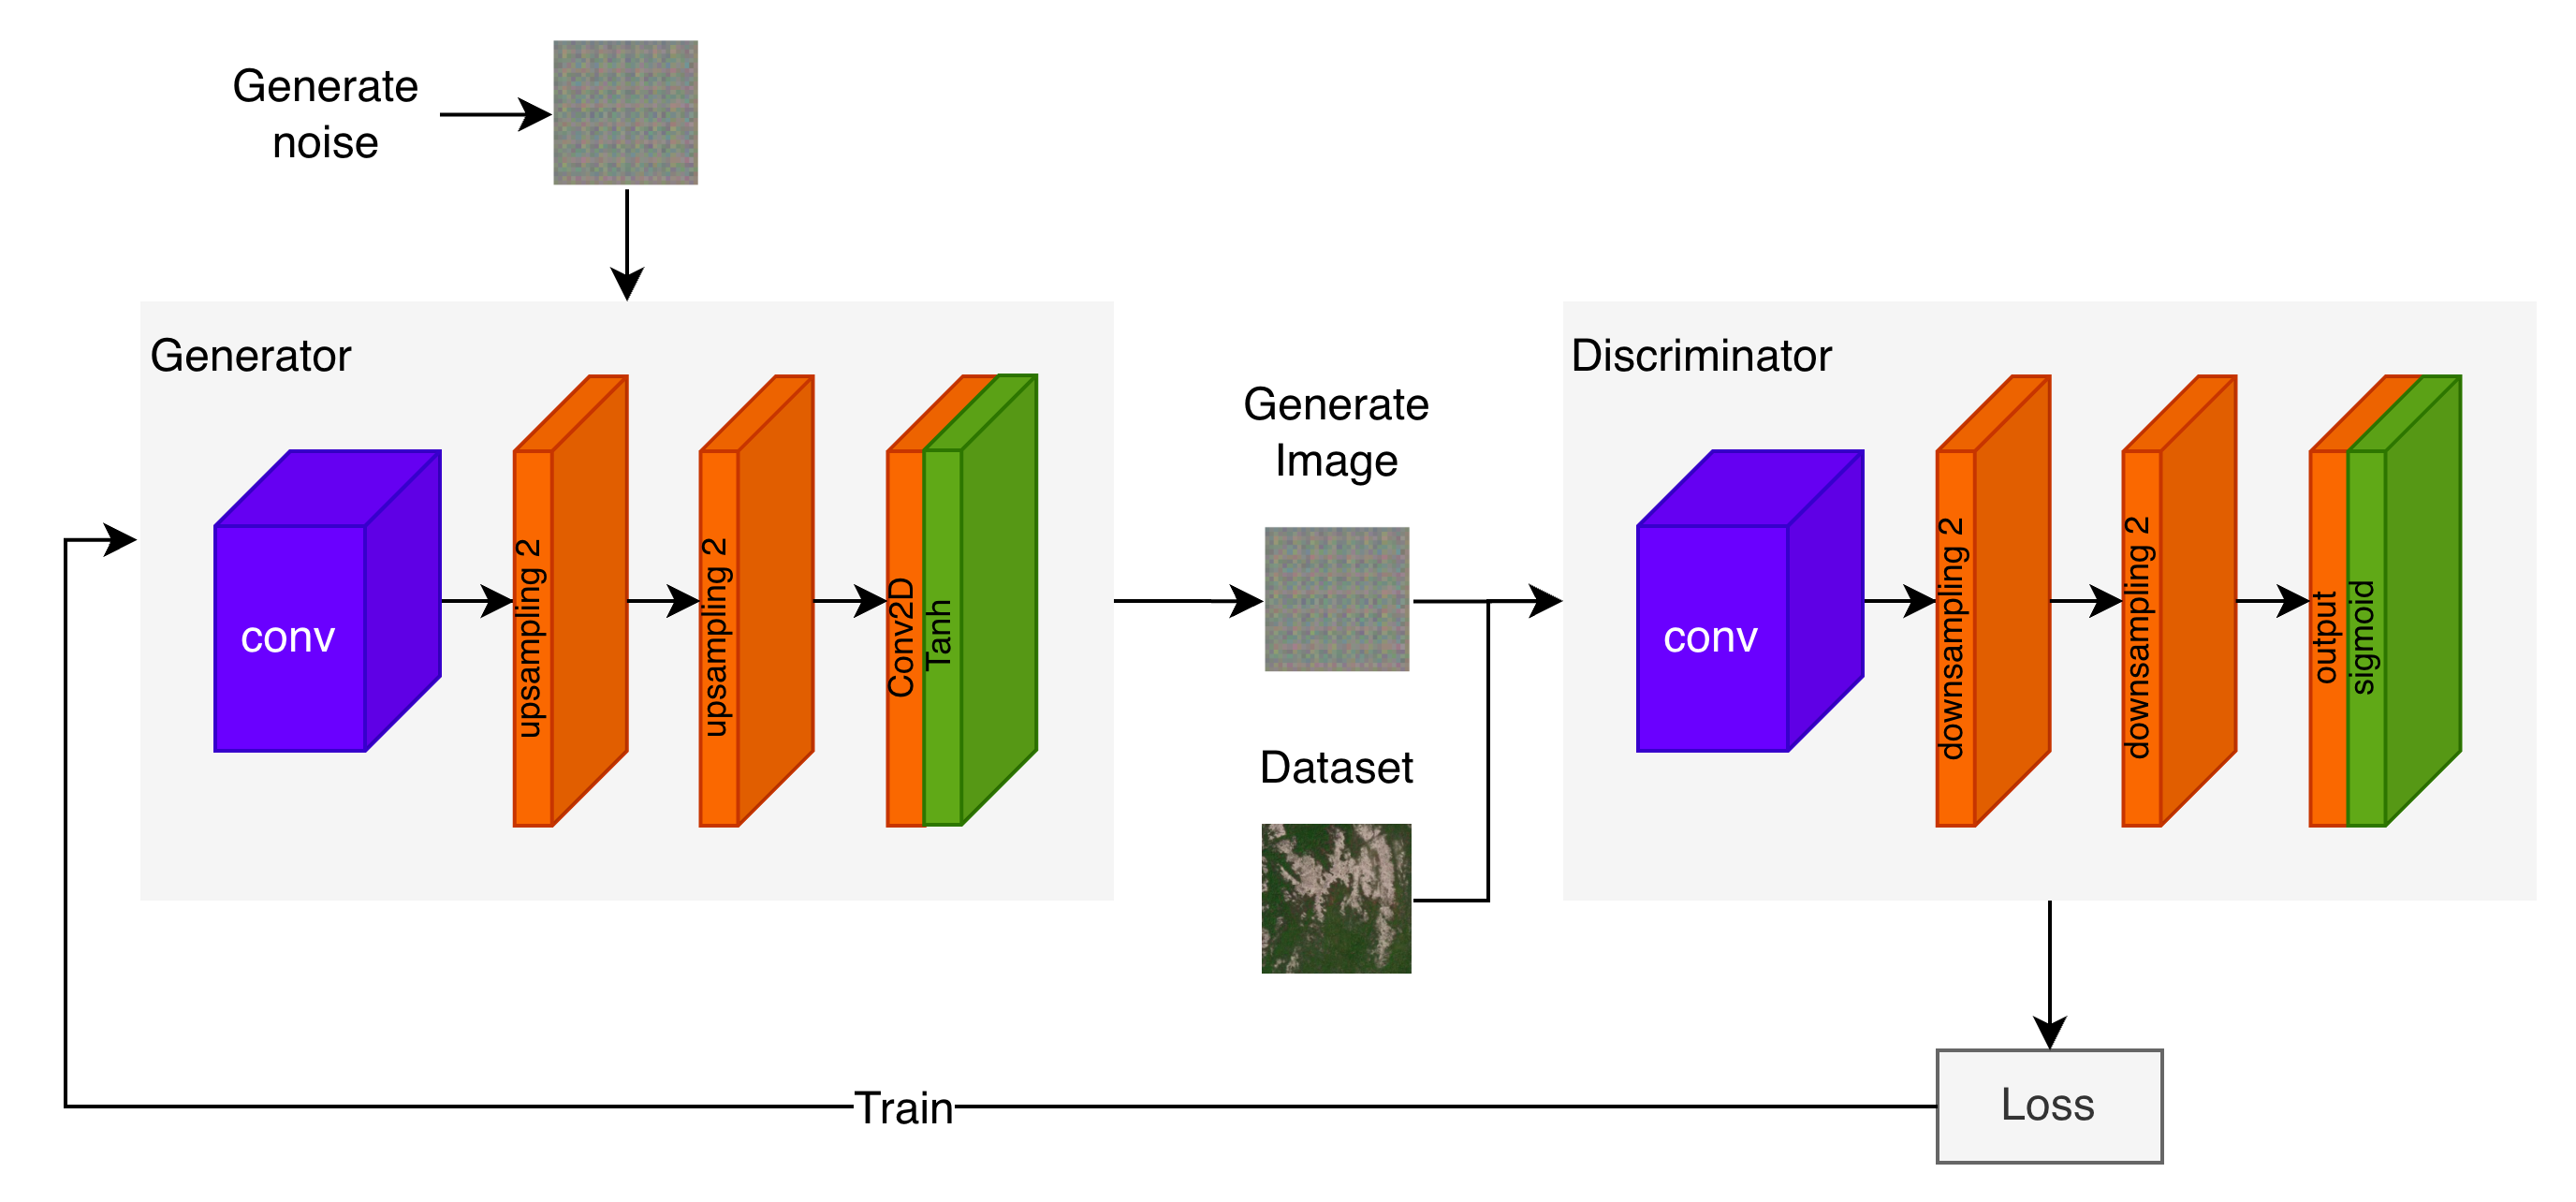
\includegraphics[width=0.8\textwidth]{gan.png}
    \caption{GAN architecture}\label{fig:gan}
\end{figure}

The classifier is using CNN based model with architecture can be seen in figure~\ref*{fig:classifier}
\begin{figure}[H]
    \centering
    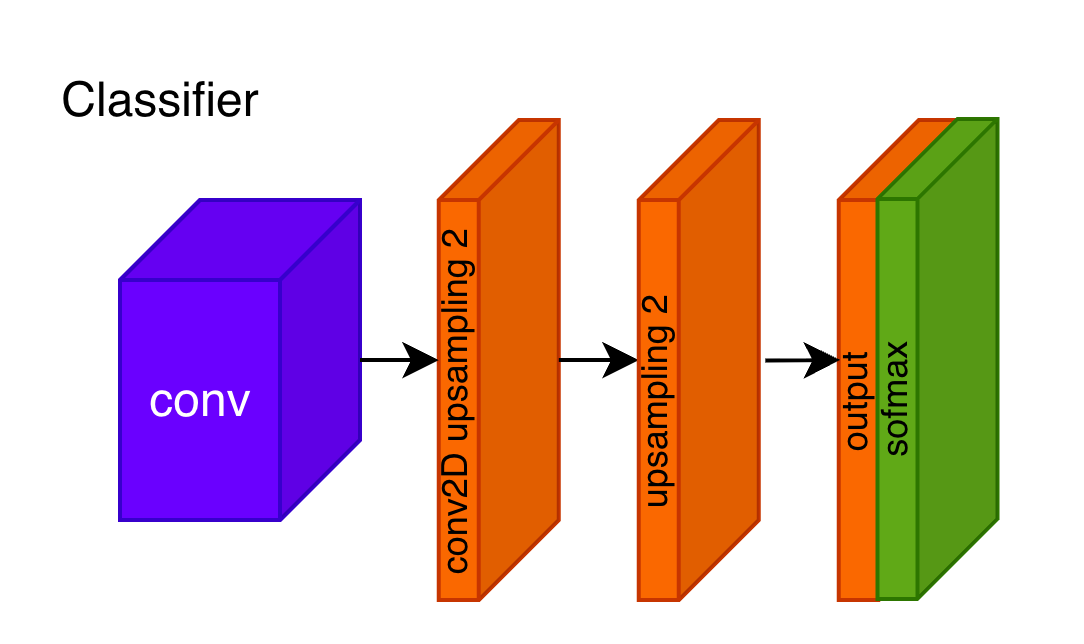
\includegraphics[width=0.8\textwidth]{classifier.png}
    \caption{Classifier architecture}\label{fig:classifier}
\end{figure}

\section{Model Evaluation}

Evaluation used in this research follows a classic binary classification problem, using binary cross entropy (BCE) to measure how well a model's predicted probabilities match to the true binary labels. 
The BCE loss decreases as the predicted probabilities closer to the true label and the increase as the predicted deviate.
\begin{equation}
    \mathcal{L}_{\text{BCE}}(y, \hat{y}) = -\left[y\log(\hat{y}) + (1 - y)\log(1 - \hat{y})\right]
\end{equation}

\section{Result}
\subsection{GAN loss and accuracy}
GAN training result in accuracy of discriminator and reduce the loss of generator. 
The result can be seen in figure~\ref*{fig:gan_results}, it shows the lastest accuracy of the discriminator is \textbf{96.99\%} and the loss function of generator is \textbf{0.4251}
\begin{figure}[H]
    \centering
    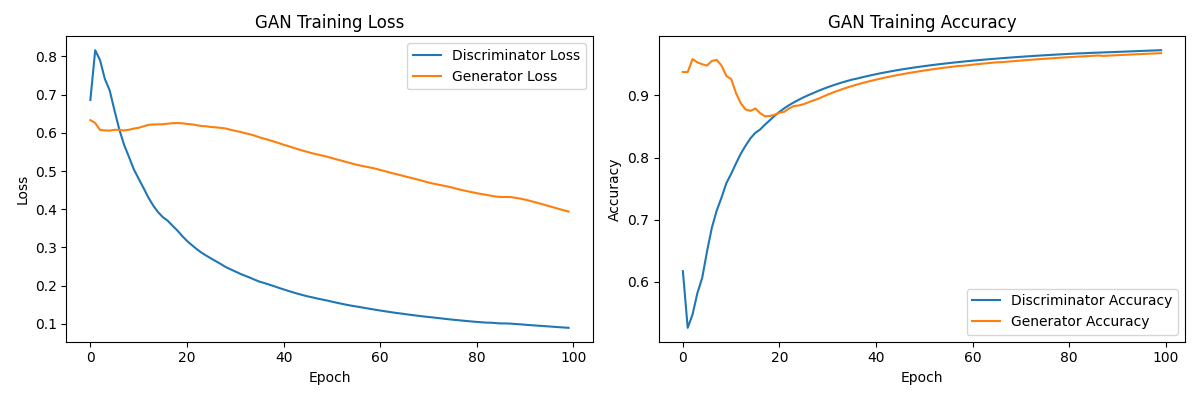
\includegraphics[width=0.8\textwidth]{gan_results.png}
    \caption{GAN result}\label{fig:gan_results}
\end{figure}

\subsection{GAN synthetic data}
The purpose of the GAN training is to create synthetic data, the example of synthetic data can be seen in figure~\ref*{fig:generated_images}.
\begin{figure}[H]
    \centering
    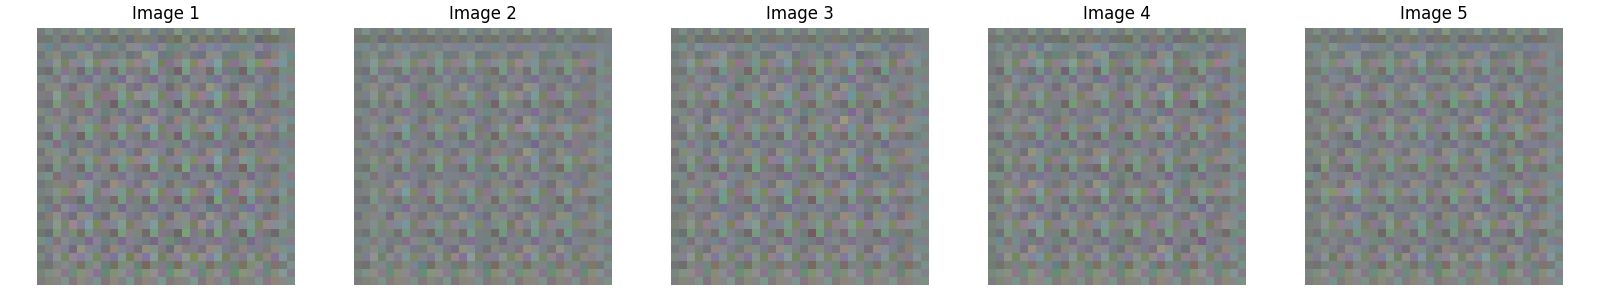
\includegraphics[width=0.8\textwidth]{generated_images.png}
    \caption{GAN generated data}\label{fig:generated_images}
\end{figure}

\subsection{Classifier training}
The classifier model is used to classify the data into binary class wildfire or not.
The training process can be seen in figure~\ref*{fig:training_history}
\begin{figure}[H]
    \centering
    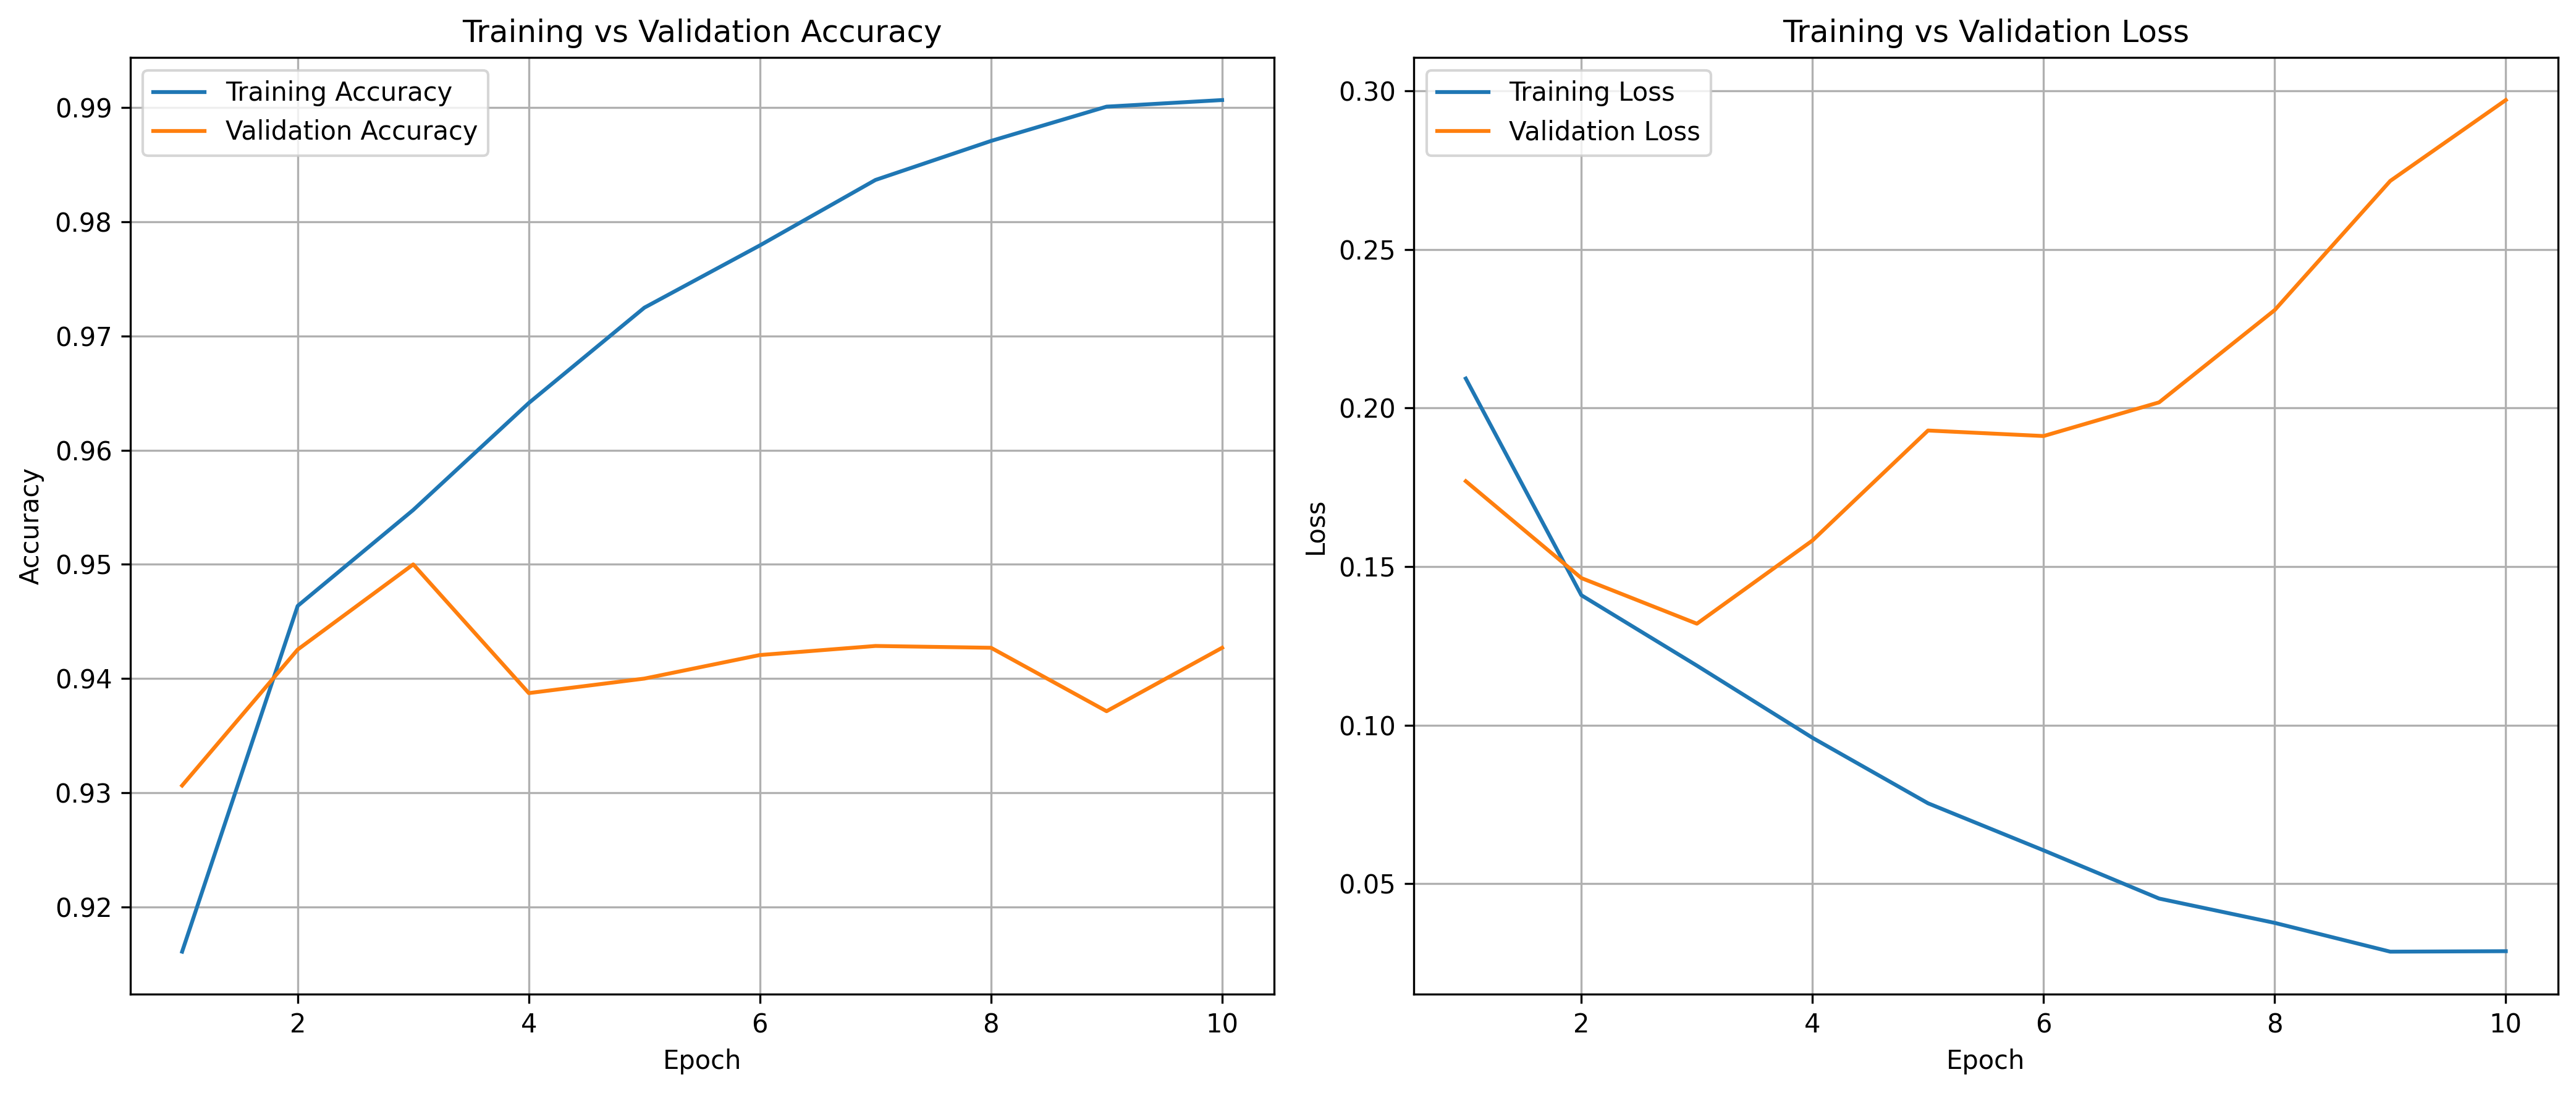
\includegraphics[width=0.8\textwidth]{training_history.png}
    \caption{Classifier training history}\label{fig:training_history}
\end{figure}

The training result shows the lastest accuracy of training dataset is \textbf{0.9907} and validation dataset is \textbf{0.9427}.
The loss function is \textbf{0.0292} for the training dataset and validation is \textbf{0.2971}.

\subsection{Classifier testing}
The testing result for classification can be seen in the confusion matrix in figure~\ref*{fig:confusion_matrix}
\begin{figure}[H]
    \centering
    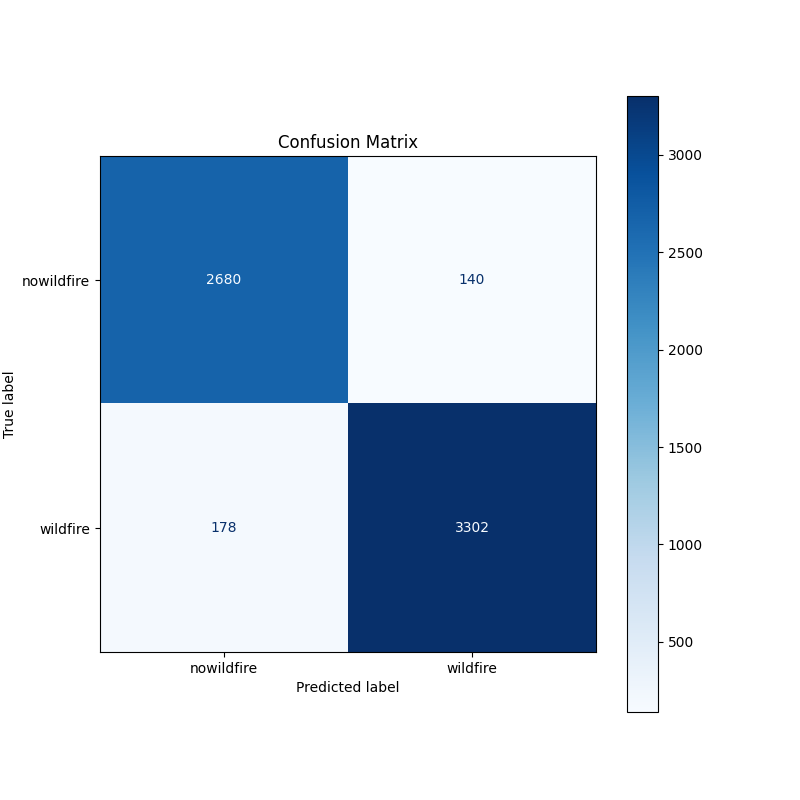
\includegraphics[width=0.8\textwidth]{confusion_matrix.png}
    \caption{Confusion matrix}\label{fig:confusion_matrix}
\end{figure}

Using accuracy, f1-score, recall and precission the result is shown in table~\ref{tab:classification_metrics}.
The overall accuracy is \textbf{94.95\%} and the result can be said to be successful to classify the wildfire problem.

\begin{table}[h]
\centering
\begin{tabular}{|l|c|c|c|c|c|}
\hline
\textbf{Class} & \textbf{Accuracy} & \textbf{Precision} & \textbf{Recall} & \textbf{F1-Score} & \textbf{Support} \\ \hline
nowildfire & 95.03 & 93.77 & 95.04 & 94.40 & 2820 \\ \hline
wildfire & 94.88 & 95.93 & 94.89 & 95.41 & 3480 \\ \hline
Overall & 94.95 & 94.97 & 94.95 & 94.96 & 6300 \\ \hline
\end{tabular}
\caption{Classification Metrics Per Class}
\label{tab:classification_metrics}
\end{table}

\subsection{Web page}
This experiment also create a web page to test the prediction model which can be seen in figure~\ref{fig:web}
\begin{figure}[H]
    \centering
    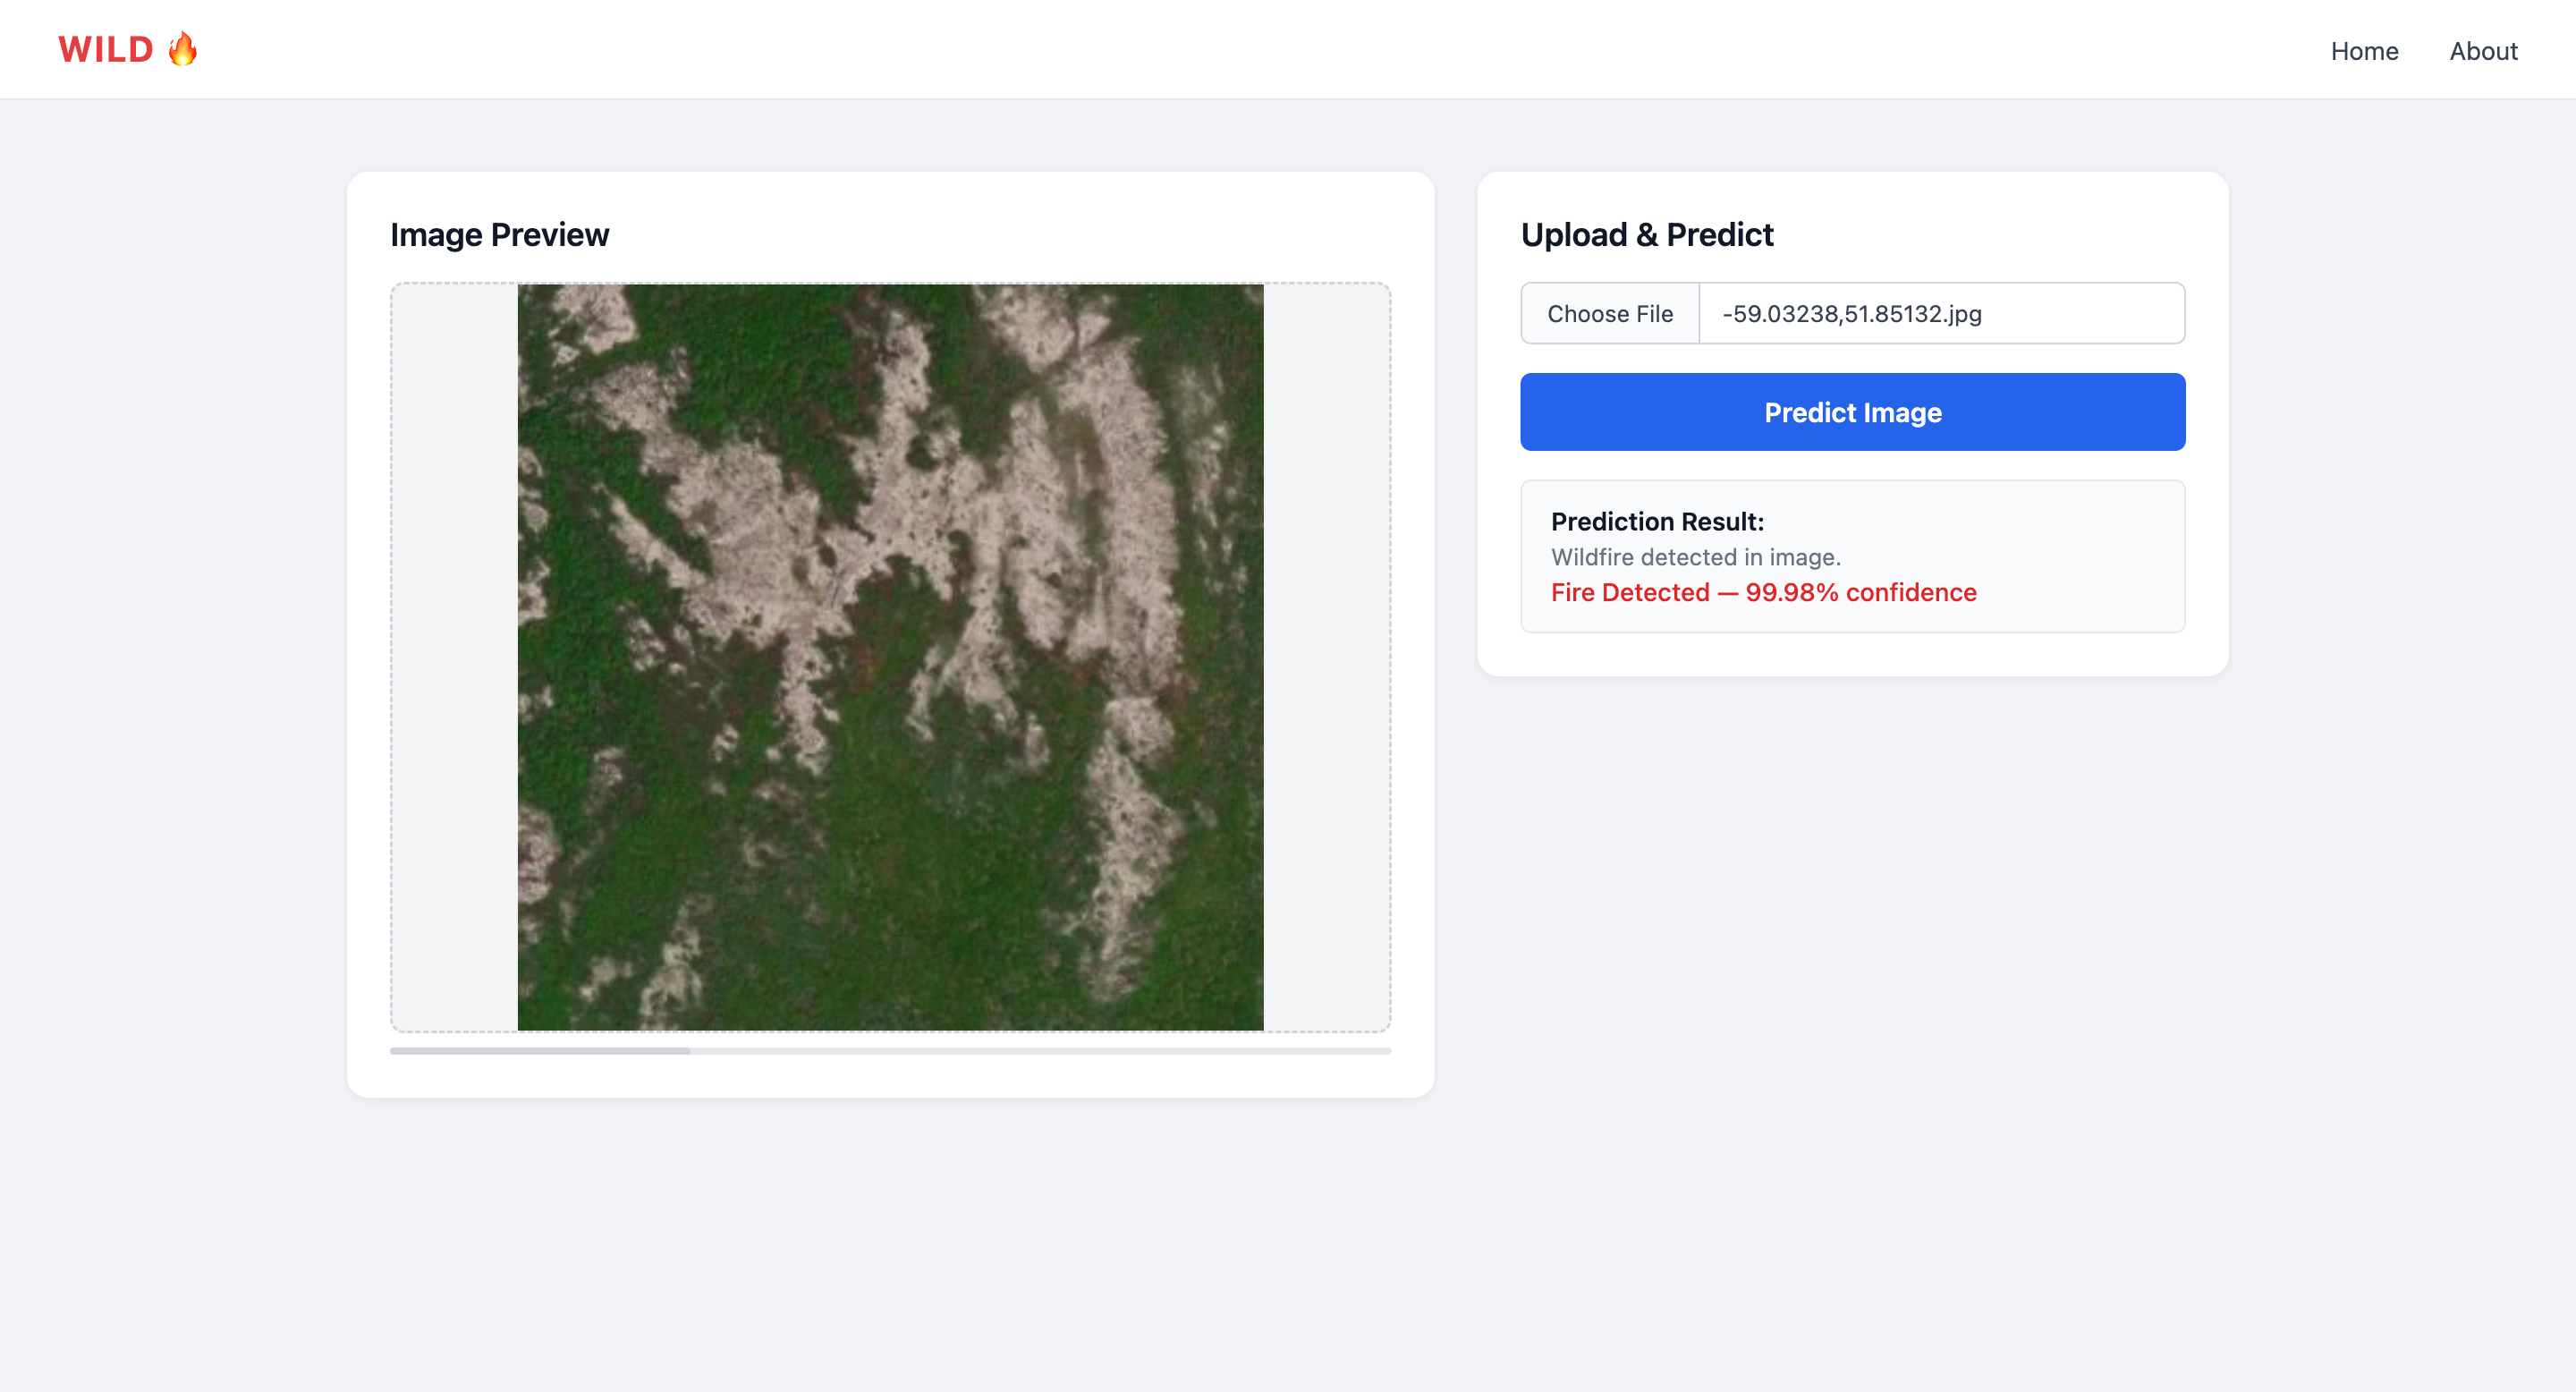
\includegraphics[width=0.8\textwidth]{web.png}
    \caption{Web}\label{fig:web}
\end{figure}

\section{Conclussion}
This implementation finds that a wildfire detection system based on Generative Adversarial Networks (GANs) can achieve strong performance while remaining practical for real-world use. 
The proposed method successfully improves the training dataset and enhances the generalization ability of classification without relying on overly complex architectures. 

This method uses synthetic data generated by GANs. The results from training and testing show that the model achieves an overall accuracy of approximately 94.95\% with balanced precision, recall, and F1 scores in forest fire and non-forest fire classes. 
This indicates that reliable forest fire detection from satellite images is still possible even with lower image resolution and simplified model design.

\end{document}